%% Creator: Inkscape inkscape 0.48pre0, www.inkscape.org
%% PDF/EPS/PS + LaTeX output extension by Johan Engelen, 2010
%% Accompanies image file 'VideoCommunication' (pdf, eps, ps)
%%
%% To include the image in your LaTeX document, write
%%   \input{<filename>.tex}
%%  instead of
%%   \includegraphics{<filename>.pdf}
%% To scale the image, write
%%   \def{\svgwidth}{<desired width>}
%%   \input{<filename>.tex}
%%  instead of
%%   \includegraphics[width=<desired width>]{<filename>.pdf}

\begingroup
  \makeatletter
  \providecommand\color[2][]{%
    \errmessage{(Inkscape) Color is used for the text in Inkscape, but the package 'color.sty' is not loaded}
    \renewcommand\color[2][]{}%
  }
  \providecommand\transparent[1]{%
    \errmessage{(Inkscape) Transparency is used (non-zero) for the text in Inkscape, but the package 'transparent.sty' is not loaded}
    \renewcommand\transparent[1]{}%
  }
  \providecommand\rotatebox[2]{#2}
  \ifx\svgwidth\undefined
    \setlength{\unitlength}{340.1574707pt}
  \else
    \setlength{\unitlength}{\svgwidth}
  \fi
  \global\let\svgwidth\undefined
  \makeatother
  \begin{picture}(1,0.91666673)%
    \put(0,0){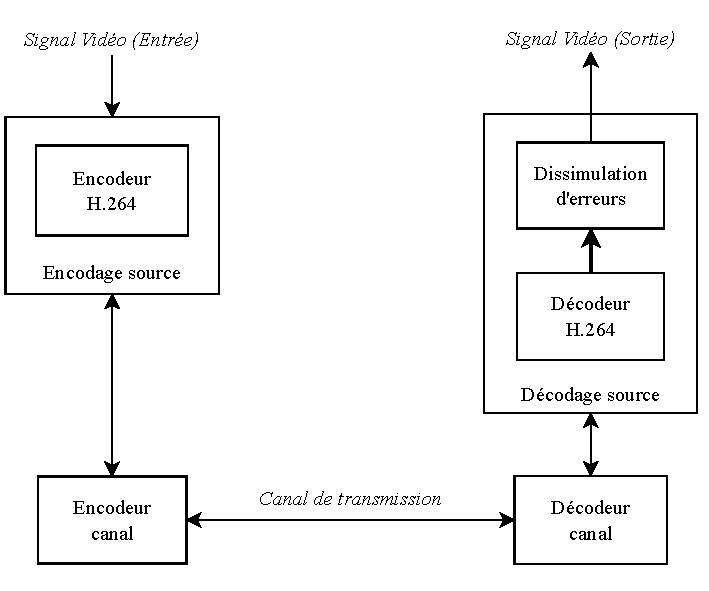
\includegraphics[width=\unitlength]{VideoCommunication}}%
    \put(0.50094847,0.21106724){\color[rgb]{0,0,0}\makebox(0,0)[b]{\smash{Canal de transmission}}}%
    \put(0.1602721,0.19871103){\color[rgb]{0,0,0}\makebox(0,0)[b]{\smash{Encodeurcanal}}}%
    \put(0.8444206,0.19731619){\color[rgb]{0,0,0}\makebox(0,0)[b]{\smash{Décodeurcanal}}}%
    \put(0.16027295,0.53344066){\color[rgb]{0,0,0}\makebox(0,0)[b]{\smash{Encodage source}}}%
    \put(0.1602721,0.66856212){\color[rgb]{0,0,0}\makebox(0,0)[b]{\smash{EncodeurH.264}}}%
    \put(0.8444206,0.35919171){\color[rgb]{0,0,0}\makebox(0,0)[b]{\smash{Décodage source}}}%
    \put(0.8444206,0.48873251){\color[rgb]{0,0,0}\makebox(0,0)[b]{\smash{DécodeurH.264}}}%
    \put(0.8444206,0.67585826){\color[rgb]{0,0,0}\makebox(0,0)[b]{\smash{Dissimulationd'erreurs}}}%
    \put(0.8444206,0.86820375){\color[rgb]{0,0,0}\makebox(0,0)[b]{\smash{Signal Vidéo (Sortie)}}}%
    \put(0.16027295,0.8669162){\color[rgb]{0,0,0}\makebox(0,0)[b]{\smash{Signal Vidéo (Entrée)}}}%
  \end{picture}%
\endgroup
